\chapter{Experiments\label{chap:experiments}}

This chapter discusses the various experiments conducted on the dataset and their results. We will first go through techniques used to train various models and then the metrics used to compare the results.

\section{Training Experiments}

As mentioned in Chapter~\ref{chap:dataset}, we don't have a balanced dataset. The number of malware samples are much greater than the benign samples. Due to this, we use cross-validation technique to train and test our machine learning models on our imbalanced dataset.

\section{Data Analysis}

As seen in Figure~\ref{fig:orig-port-freq}, initial data analysis reveals that the most frequent ports in malware captures are different than the most frequent ports in the benign captures. Similar result can be seen in Figure~\ref{fig:resp-port-freq} which is a plot of the port number frequencies used by the responding endpoint in the network traffic capture. The top 5 ports with the highest frequency in both the captures are shown in Table~\ref{tab:5} and Table~\ref{tab:6}.

\begin{figure}[htb]
	\centering
	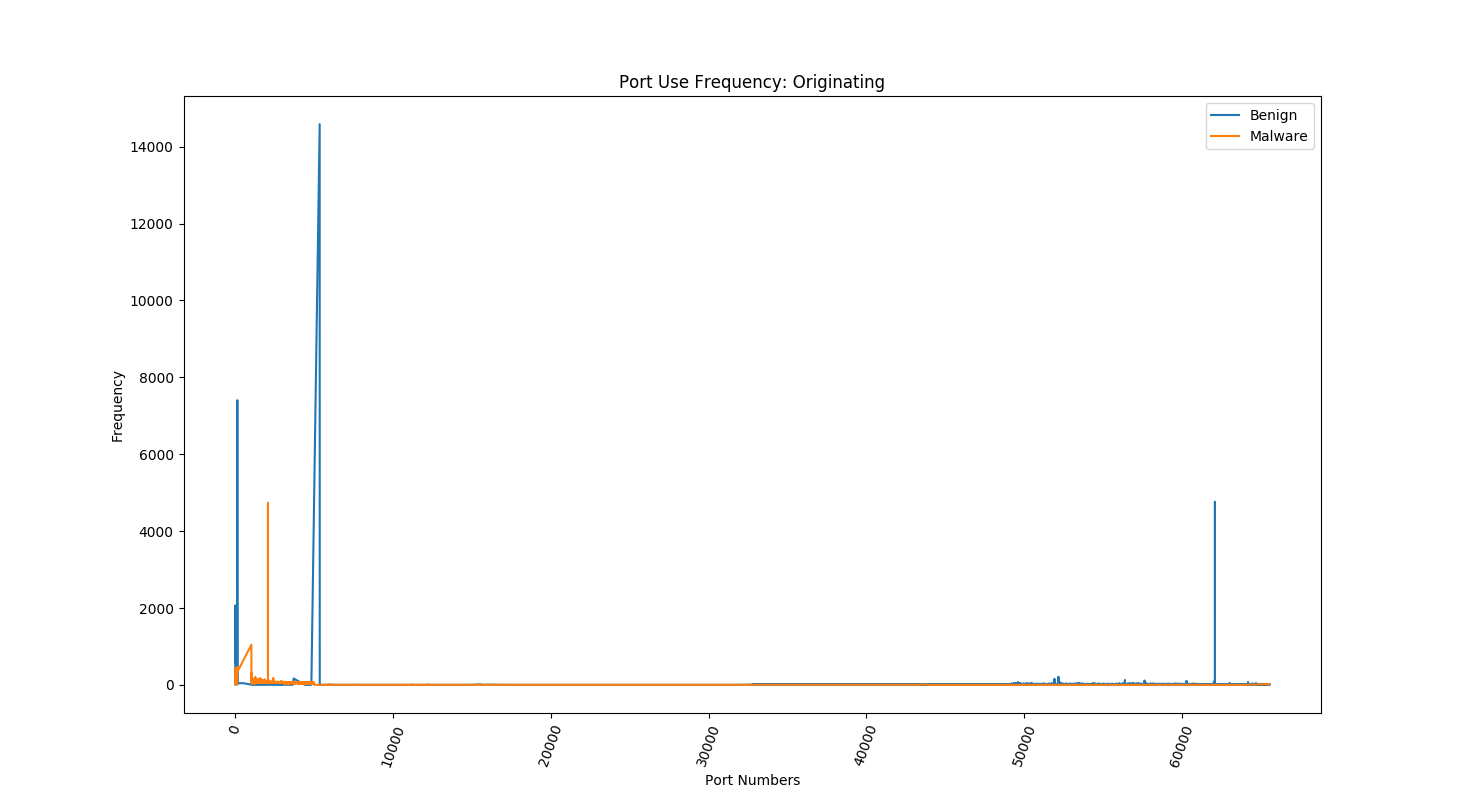
\includegraphics[width=1\textwidth]{images/orig-port-freq.png}
	\caption{Frequency of ports used by ORIG} 
	\label{fig:orig-port-freq}
\end{figure}

\begin{figure}[htb]
	\centering
	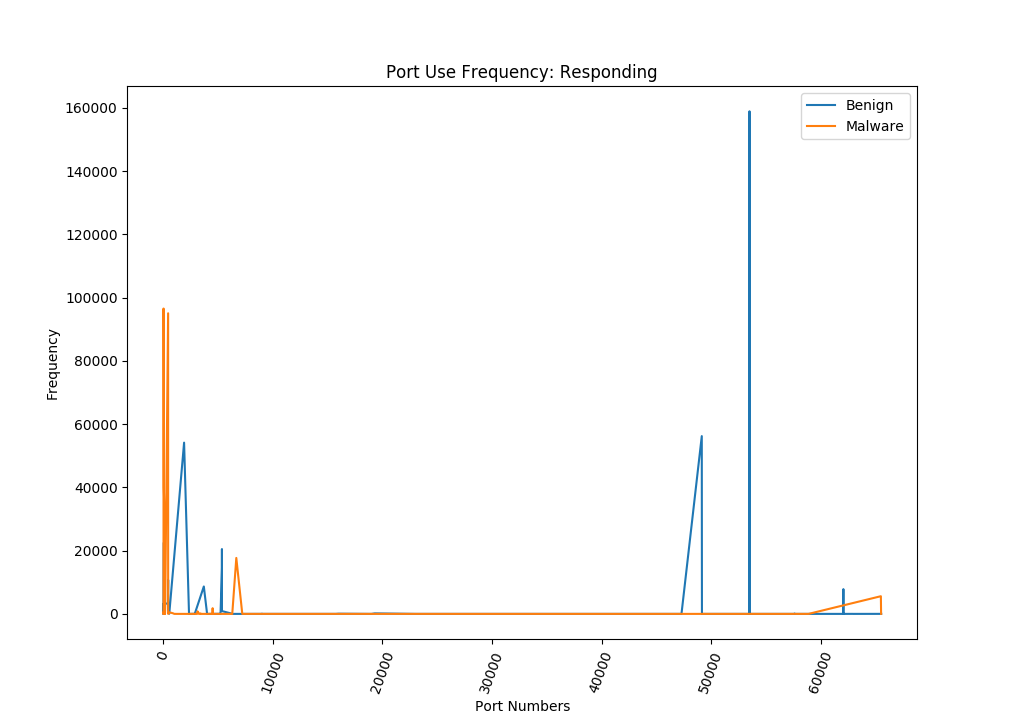
\includegraphics[width=1\textwidth]{images/resp-port-freq.png}
	\caption{Frequency of ports used by RESP} 
	\label{fig:resp-port-freq}
\end{figure}

\begin{table}[!htb]
	\caption{Top Five Ports Used by ORIG\label{tab:5}}
	\begin{center}
		\begin{tabular}{c|p{0.15\textwidth}|p{0.50\textwidth}}\hline\hline
			Dataset & Port Number & \multicolumn{1}{l}{Known Port Assignments} \\ \hline
			Malware & 2077 & WebDisk or Old Tivoli Storage \\
			& 2079	&  IDWARE Router Port\\
			& 1025	&  Ports > 1024 are designated for dynamic allocation by Windows\\
			& 137	&  File and Print Sharing under Windows\\
			& 3 &  Compression Process \\ \hline
			Benign & 5353  &  Multicast DNS, iChat, Mac OS X Bonjour\\
			& 135 &  Remote Procedure Call (RPC)\\
			& 62078 &  UPnP (Universal Plug and Play), iTunes\\
			& 137 &  File and Print Sharing under Windows\\
			& 138 &  File and Print Sharing under Windows\\
			\hline\hline
		\end{tabular}
	\end{center}
\end{table}

\begin{table}[!htb]
	\caption{Top Five Ports Used by RESP\label{tab:6}}
	\begin{center}
		\begin{tabular}{c|p{0.15\textwidth}|p{0.50\textwidth}}\hline\hline
			Dataset & Port Number & \multicolumn{1}{l}{Known Port Assignments} \\ \hline
			Malware & 25 & SMTP (Simple Mail Transfer Protocol) \\
			& 443	&  HTTPS / SSL - encrypted web traffic\\
			& 53	&  DNS (Domain Name Service)\\
			& 80	&  Hyper Text Transfer Protocol (HTTP) \\
			& 6667 &  IRC (Internet Relay Chat) \\ \hline
			Benign & 53508  &  Xsan Filesystem Apple\\
			& 49153 &  ANTLR, ANother Tool for Language Recognition\\
			& 1900 &  IANA registered by Microsoft for SSDP (Simple Service Discovery Protocol)\\
			& 53 &  DNS (Domain Name Service)\\
			& 5355 &  Link-Local Multicast Name Resolution Windows\\
			\hline\hline
		\end{tabular}
	\end{center}
\end{table}

As we can see from Table~\ref{tab:5} and Table~\ref{tab:6}, malware dataset had Internet Relay Chat (IRC) port among the most frequently used. We know that most of the malware use IRC to exfiltrate data from the infected system to other systems. We also see that HTTPS port 443 is also among the most frequently used in the malware captures.

\pagebreak

\section{K-means Clustering}

K-means clustering is an unsupervised learning algorithm that aims to partition \verb|n| data points into \verb|k| clusters. Clustering is used to see whether the data points naturally form distinct clusters or whether they are similar to other data points in the dataset. We normalized the values in our dataset and performed K-means clustering with \verb|k=2|. The results are shown in Figure~\ref{fig:kmeans1} and Figure~\ref{fig:kmeans2} below.

\begin{figure}[htb]
	\centering
	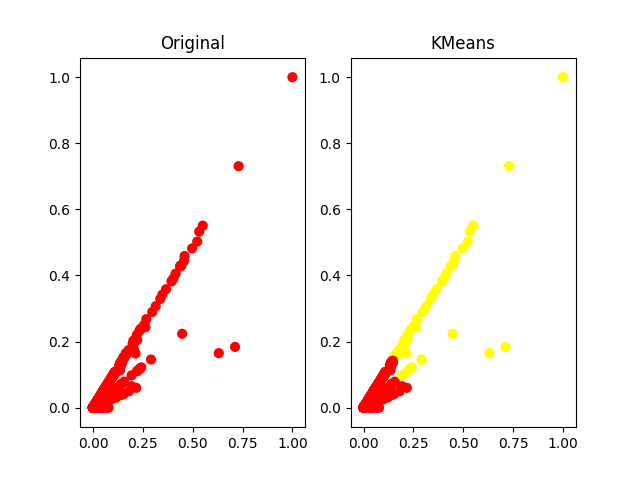
\includegraphics[width=1\textwidth]{images/kmeans.png}
	\caption{Original Scatter Plot vs K-means clustering} 
	\label{fig:kmeans1}
	
	\centering
	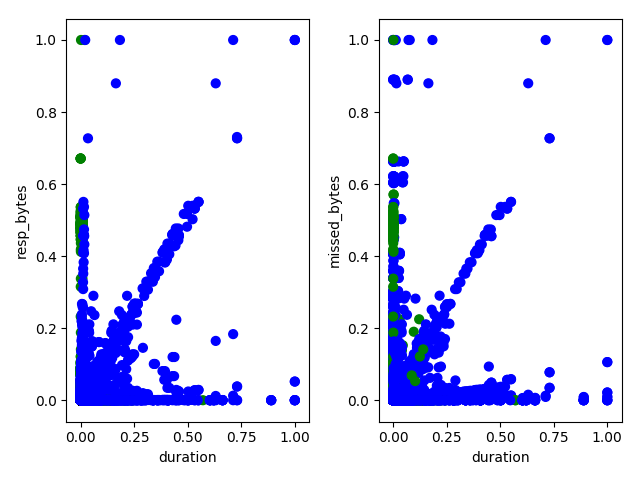
\includegraphics[width=1\textwidth]{images/kmeans2.png}
	\caption{Original Scatter Plots with different axes} 
	\label{fig:kmeans2}
\end{figure}

As seen in Figure~\ref{fig:kmeans1}, K-means didn't really give us distinct clusters. Also , most of the scatter plots based on connection features resemble that in Figure~\ref{fig:kmeans2}. We further perform experiments using Support Vector Machine (SVM) and univariate feature analysis to find prominent features in the dataset.

\clearpage

\section{Experiments}

This section states multiple experiments conducted using various machine learning techniques and discusses the results. 

\subsection{Experiment 1}

In this experiment we ran SVM with linear kernel and 10-fold cross validation on our dataset and achieved an average accuracy rate of $92.07$\% as shown in Figure~\ref{fig:result_svm}.

\begin{figure}[htb]
	\centering
	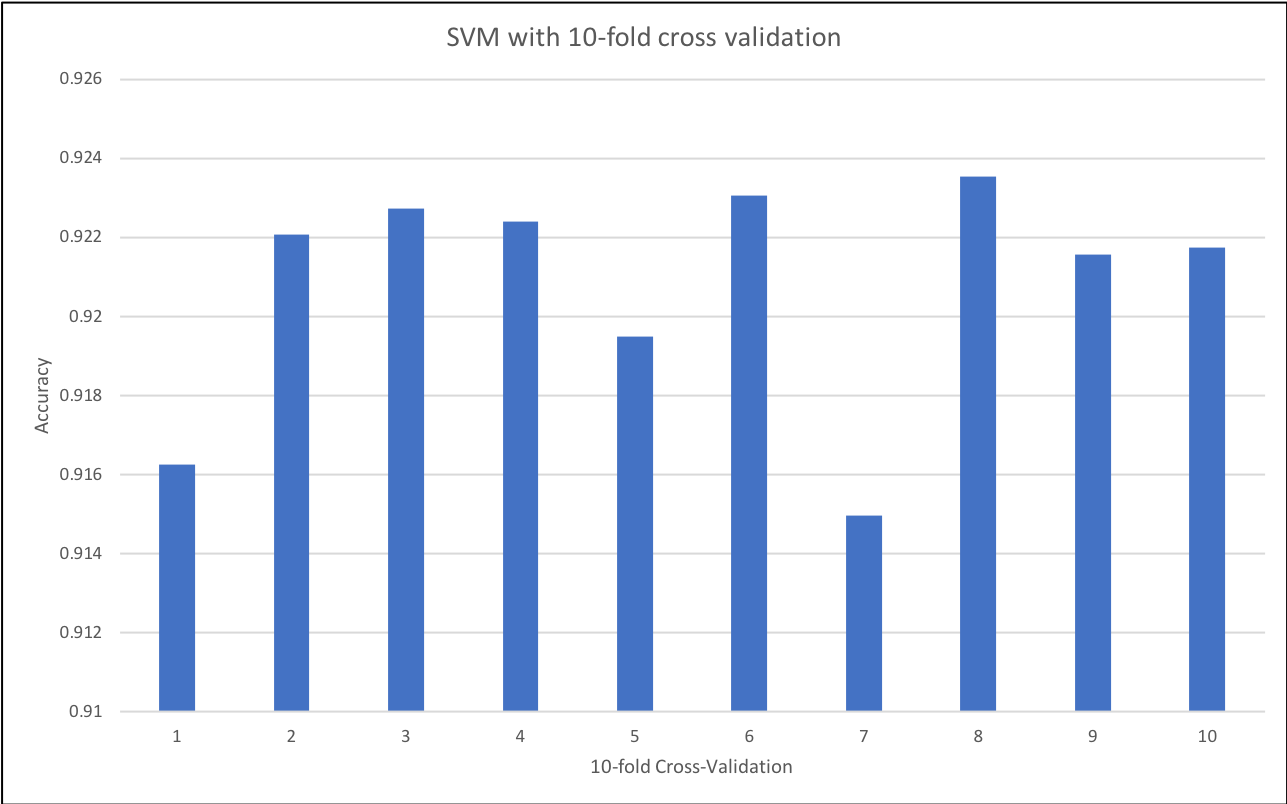
\includegraphics[width=0.7\textwidth]{images/svm.png}
	\caption{SVM with 10-fold cross-validation} 
	\label{fig:result_svm}
\end{figure}

SVM also assigns weights to the input features which provided an insight into the features SVM believes are important. In Figure~\ref{fig:result_svm_weights}, we can see that SVM assigned the highest weight to feature number 16 which is the average certificate length. Table~\ref{tab:7} provides us the rank assigned to each feature by SVM. We can see that average certificate length, periodicity and average public key length are the top most features. Also from~\cite{AndersonM16} we know that malware use weak encryption techniques such as shorter key lengths and are more periodic in nature than other applications. Also, the validity of certificate during capture is the sixth highest rank feature which tell us that most of malware may not have a valid certificate.

 \begin{figure}[htb]
 	\centering
 	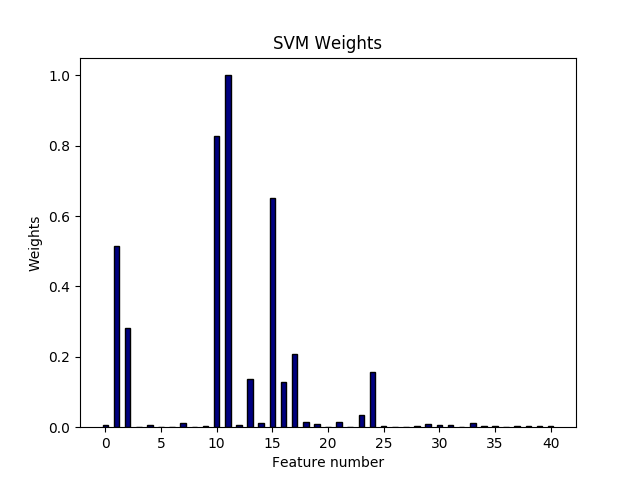
\includegraphics[width=1\textwidth]{images/svm_weights.png}
 	\caption{Weights assigned to features by SVM} 
 	\label{fig:result_svm_weights}
 \end{figure}

\begin{table}[!htb]
	\caption{Feature ranks by SVM \label{tab:7}}
	\begin{center}
		\begin{tabular}{c|p{0.50\textwidth}}\hline\hline
			Rank & Feature  \\ \hline
			 1  & average\_of\_certificate\_length           \\
			 2  & periodicity\_standard\_deviation           \\
			 3  & periodicity\_average                       \\
			 4  & standart\_deviation\_cert\_length          \\
			 5  & average\_public\_key                       \\
			 6  & is\_valid\_certificate\_during\_capture    \\
			 7  & average\_of\_duration                      \\
			 8  & standard\_deviation\_duration              \\
			 9  & self\_signed\_ratio                        \\
			 10 & SNI\_ssl\_ratio                            \\
			 11 & ratio\_of\_differ\_sandns\_in\_cert        \\
			 12 & percent\_of\_established\_states           \\
			 13 & number\_of\_certificate\_path              \\
			 14 & ratio\_of\_differ\_subject\_in\_cert       \\
			 15 & ratio\_of\_differ\_subject\_in\_ssl\_log   \\
			 16 & tls\_version\_ratio                        \\
			 17 & is\_SNI\_in\_top\_level\_domain            \\
			 18 & total\_size\_of\_flows\_orig               \\
			 19 & ratio\_of\_sizes                           \\
			 20 & ratio\_of\_differ\_issuer\_in\_ssl\_log    \\
			 21 & ratio\_of\_same\_subjects                  \\
			 22 & ratio\_of\_same\_issuer                    \\
			 23 & average\_certificate\_exponent             \\
			 24 & outbound\_pckts                            \\
			 25 & number\_of\_flows                          \\
			 26 & is\_SNIs\_in\_SNA\_dns                     \\
			 27 & ratio\_certificate\_path\_error            \\
			 28 & ratio\_missing\_cert\_in\_cert\_path       \\
			 29 & ratio\_of\_differ\_SNI\_in\_ssl\_log       \\
			 30 & inbound\_pckts                             \\
			 31 & ssl\_ratio                                 \\
			 32 & amount\_diff\_certificates                 \\
			 33 & ratio\_is\_same\_CN\_and\_SNI              \\
			 34 & number\_of\_domains\_in\_certificate       \\
			 35 & is\_CNs\_in\_SNA\_dns                      \\
			 36 & x509\_ssl\_ratio                           \\
			 37 & total\_size\_of\_flows\_resp               \\
			 38 & ratio\_of\_differ\_issuer\_in\_cert        \\
			 39 & percent\_of\_standard\_deviation\_duration \\
			 40 & certificate\_ratio                         \\
			 41 & SNI\_equal\_DstIP                        \\ \hline
		\end{tabular}
	\end{center}
\end{table}

\clearpage

\subsection{Experiment 2}

After getting the feature ranks from SVM, we also performed univariate feature elimination (UFE) to see if the feature ranks provided by SVM matches that of UFE. We ran UFE with 10-fold cross-validation and plot the ranks along with SVM ranks. As seen in Figure~\ref{fig:result_ufe_svm}, the weight rankings of UFE is almost similar to that of SVM.

\begin{figure}[htb]
	\centering
	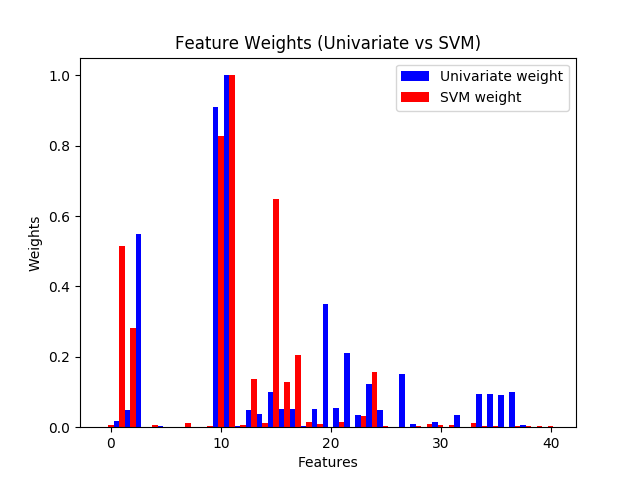
\includegraphics[width=1\textwidth]{images/ufe_svm.png}
	\caption{Weights assigned to the features by SVM and UFE} 
	\label{fig:result_ufe_svm}
\end{figure}

\subsection{Experiment 3}

After confirming the SVM feature ranks with that of UFE, we used Recursive Feature Elimination (RFE) with SVM and 10-fold cross-validation to remove weak features and calculate the accuracy. RFE iteratively eliminates one feature at a time and calculates the accuracy until just one feature remains.

As we can see from Figure~\ref{fig:result_rfe}, we get within a $2$\% of the best result with just 6 features and within $1$\% with 10 features out of 41. It shows that the top 6 features in Table~\ref{tab:5} contribute the most to the accuracy of the model.

\begin{figure}[htb]
	\centering
	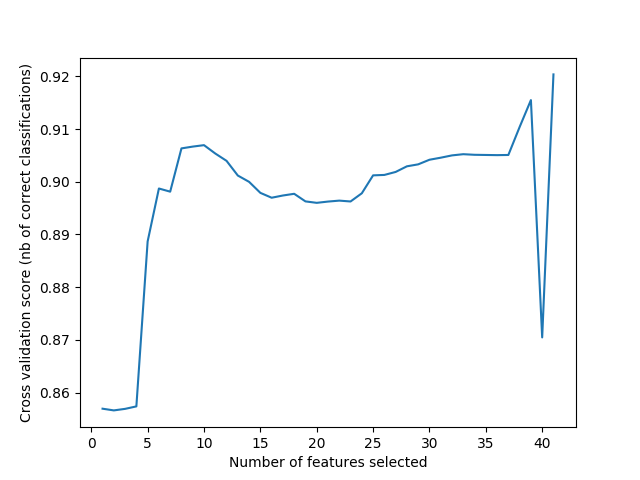
\includegraphics[width=1\textwidth]{images/rfe_svm.png}
	\caption{Recursive Feature Elimination with SVM} 
	\label{fig:result_rfe}
\end{figure}


\subsection{Experiment 4}

In this experiment we ran Random Forest Classifier with Recursive Feature Elimination and 10-fold cross-validation on the dataset to support the results given by SVM in previous section.

\begin{figure}[htb]
	\centering
	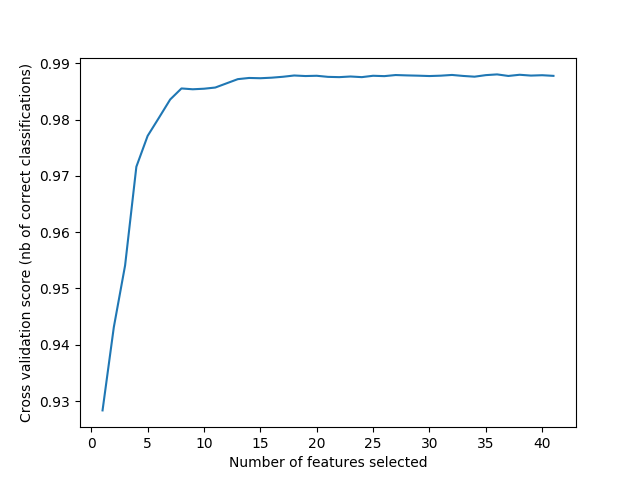
\includegraphics[width=1\textwidth]{images/rf_rfe.png}
	\caption{Recursive Feature Elimination with Random Forest} 
	\label{fig:result_rf_rfe}
\end{figure}

The first observation from Figure~\ref{fig:result_rf_rfe} is that Random Forest gives us a much higher accuracy than SVM. It also supports the SVM result that the top 6 features contribute the most to the accuracy and the remaining features can be eliminated.

\subsection{Experiment 5}

In this experiment we ran XGBoost classifier with 10-fold cross validation and compared the results to that of SVM and Random Forest.

\begin{figure}[htb]
	\centering
	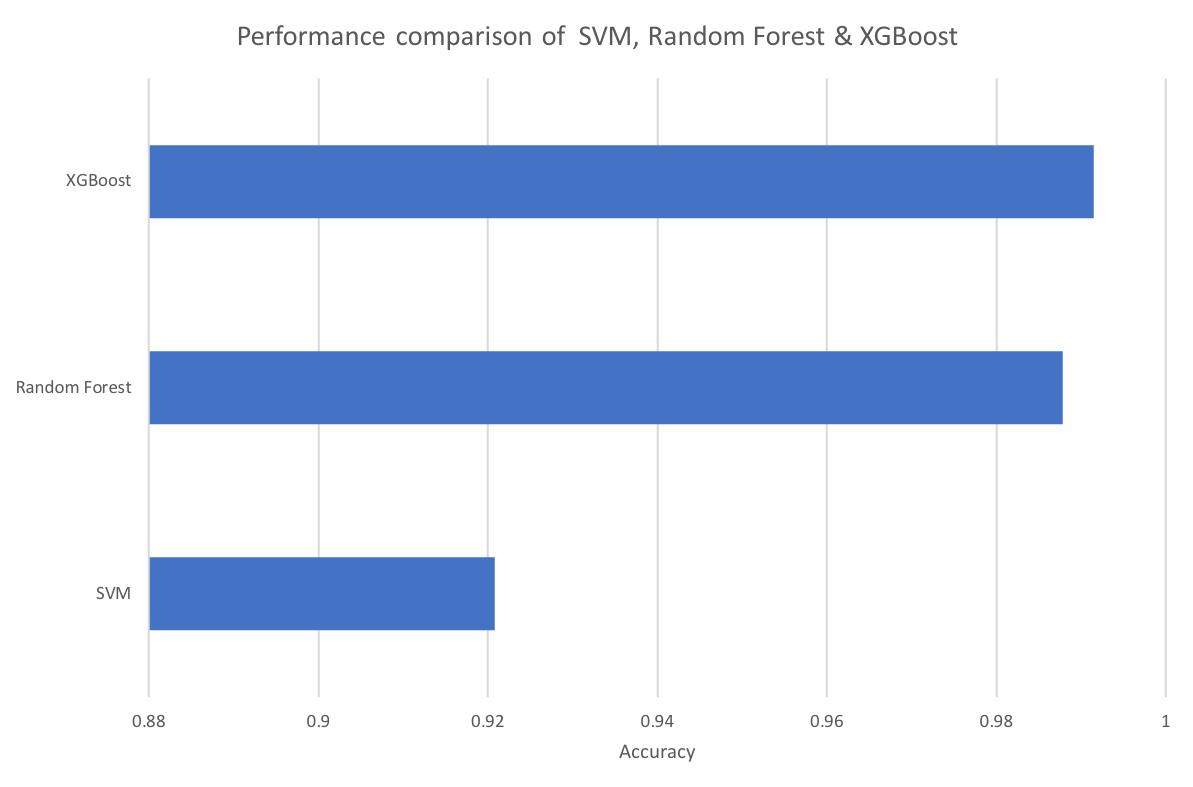
\includegraphics[width=1\textwidth]{images/svm_rf_xgb.png}
	\caption{Performance comparison of the three machine learning algorithms} 
	\label{fig:result_svm_rf_xgb}
\end{figure}

We can see that XGBoost gives us the highest accuracy of $99.15$\% followed by Random Forest which gives us an accuracy of $98.78$. Thus, we can say that ensemble techniques such as XGBoost and Random Forest performs the best on the given dataset and can be used to identify malicious encrypted traffic.

\pagebreak

\section{Discussion}

As seen in Figure~\ref{fig:ml_comparison}, XGBoost performs better than other algorithms. We get an area under the curve (AUC) value of 0.9988 for XGBoost, whereas SVM and Random Forest achieve an AUC of 0.9122 and 0.998 respectively. Thus the highest accuracy gained in our approach is 99.88\% which is the same as that achieved by Anderson and McGrew in~\cite{AndersonM17}. We achieved a constant higher accuracy for different malware samples than the other related work mentioned in Chapter~\ref{chap:related}~\cite{TegelerFVK12,PrasseMPHS17,LokocKCSP16}. As seen in Figure~\ref{fig:heatmap}, length of the encryption key, certificate length, TLS version and certificate validity are highly correlated with other features and are also the most prominent features selected by both SVM and UFE in the above experiments. This result is also supported by research carried out by Anderson and McGrew in~\cite{AndersonPM16}. In Figure~\ref{fig:heatmap}, we can also see that the corresponding columns for certificate path error, missing certificate in certificate path and SNI equal to destination IP features are missing. This is because these three features remain constant through out our dataset and as such has no affect on our classification models. Hence, these features can be removed from consideration in further research.

\begin{figure}[htb]
	\centering
	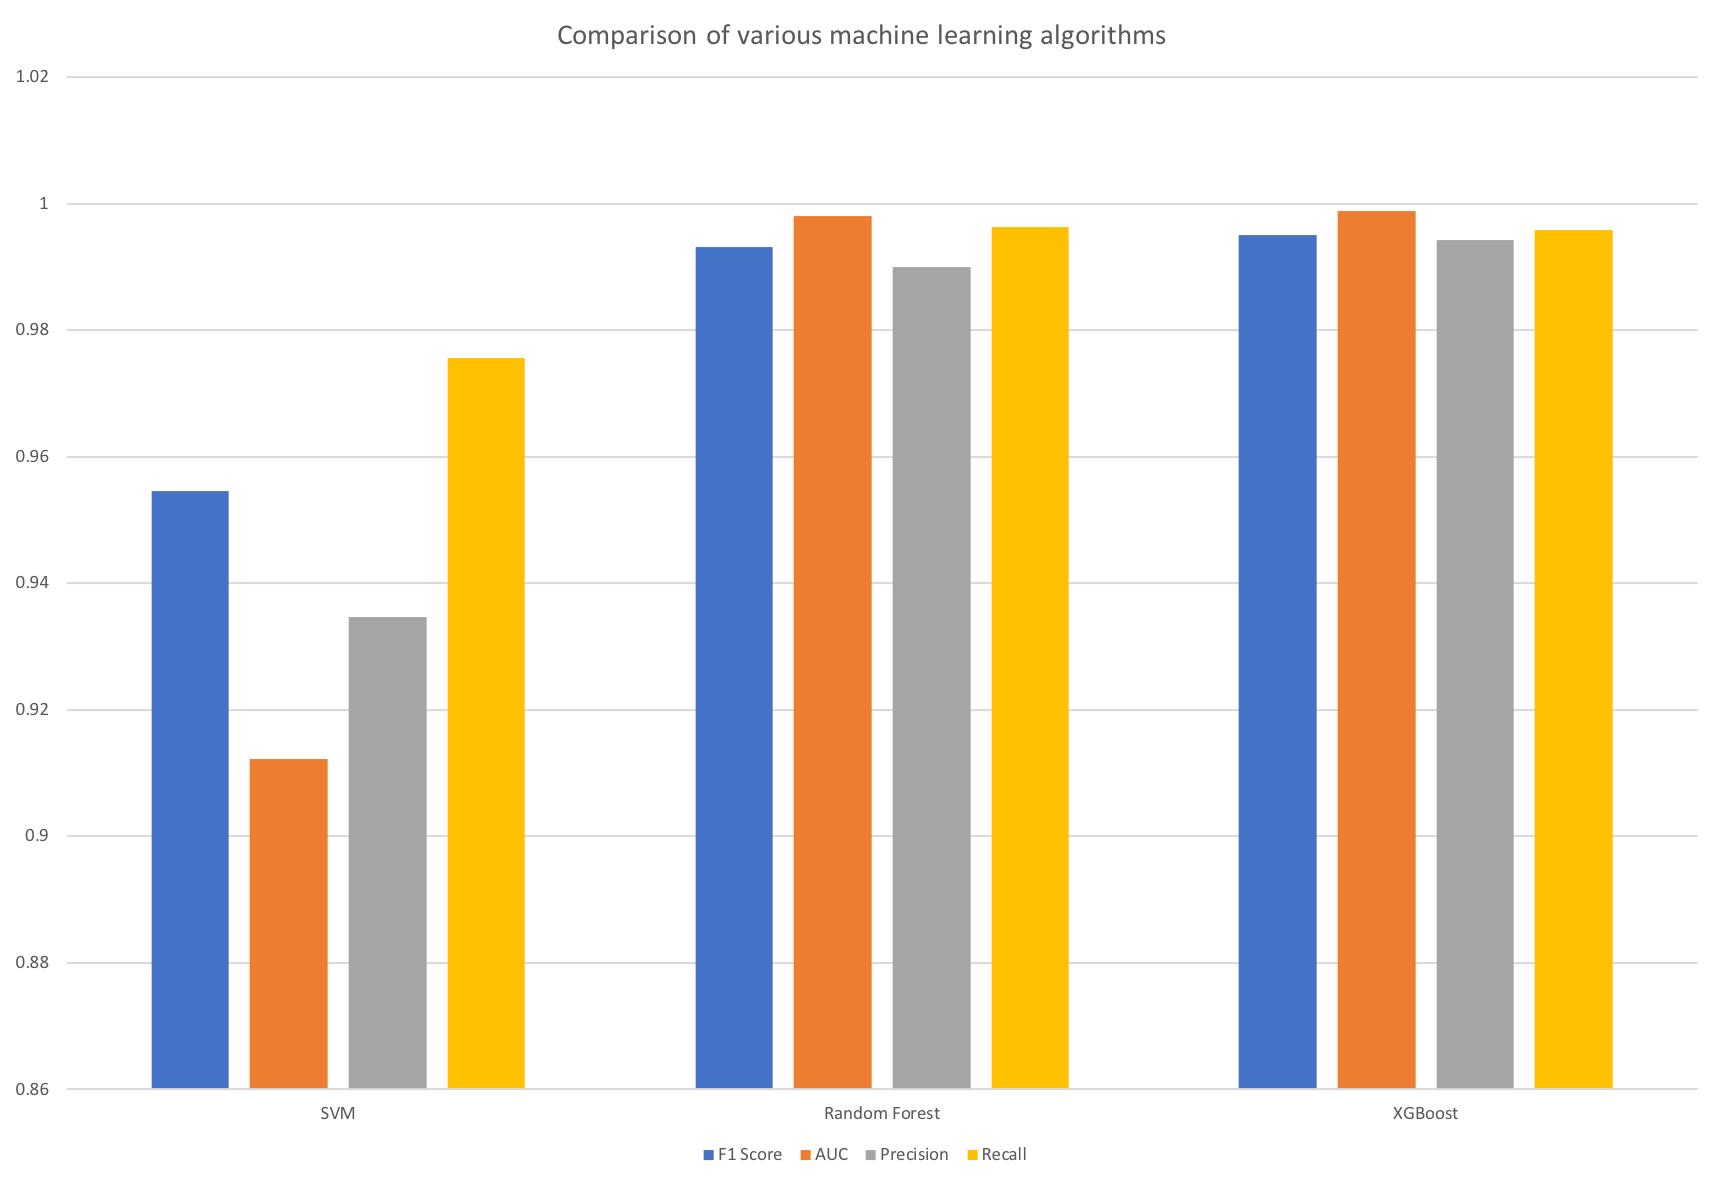
\includegraphics[width=1\textwidth]{images/ml_comparison.png}
	\caption{Comparison of various machine learning algorithms} 
	\label{fig:ml_comparison}
\end{figure}

\begin{figure}[htb]
	\centering
	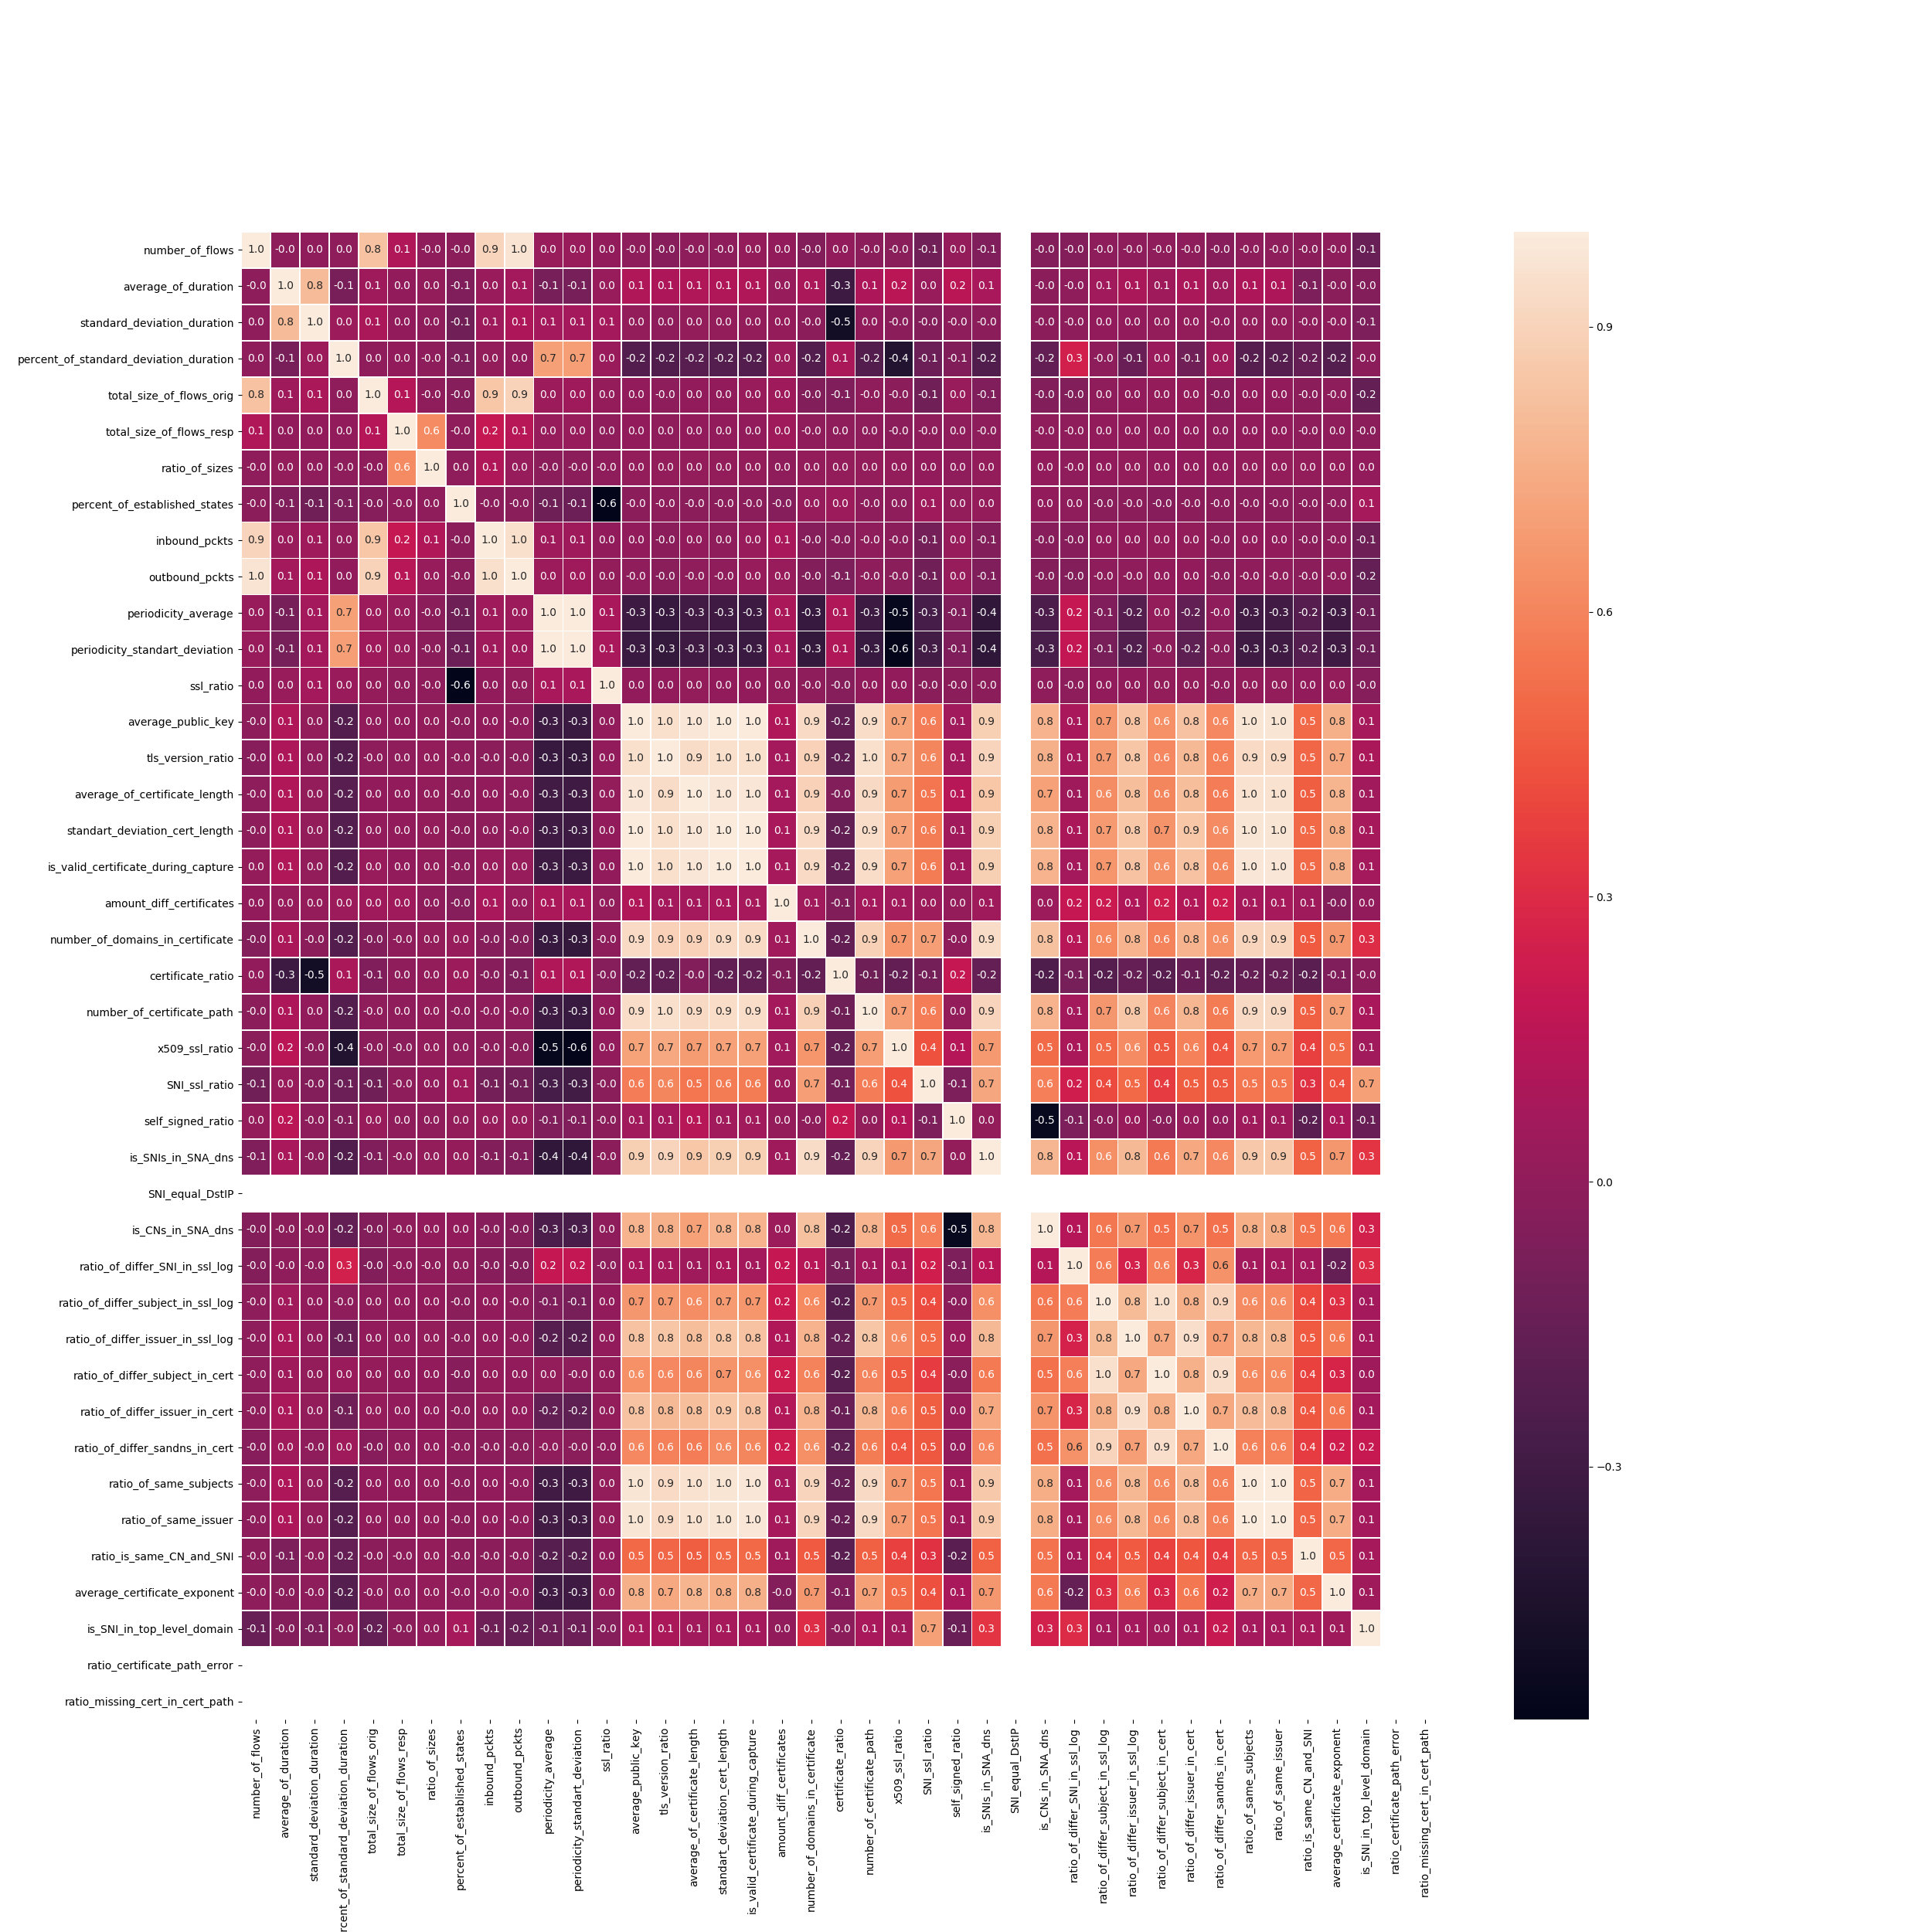
\includegraphics[width=1.2\textwidth]{images/heatmap.png}
	\caption{Feature correlation heat map} 
	\label{fig:heatmap}
\end{figure}

